\section{Development of Configuration, Data-acquisition, and Calibration Software for the Validation of the NSW Frontend}
\label{sec:nsw_vrs}

To facilitate the testing and readout of the VMM ASIC, in view of its evolution
and the approaching installation of the NSW, a complete
configuration and data-acquisition (DAQ) system has been built.
The system, referred to as the `VMM Readout System' (VRS), consists of a flexible
firmware and software infrastructure that allows for
interfacing to frontend boards housing the VMM ASIC.

A minimal instantiation of the VRS system is illustrated in Figure~\ref{fig:vrs_diagram_minimal}
in which the DAQ PC, hosting the VRS software, communicates directly to a set
of frontend boards via the network.\footnote{Network communication in the VRS system is implemented following the User Datagram Protocol (UDP) network
communication protocol. Physical network connections are made using standard Ethernet cables and on-board RJ-45 connectors.}
The frontend boards need not be interfaced to a detector, as signals can be injected via
the test-pulse injection capacitors on the VMM channels.
The firmware, loaded onto the FPGA on each frontend board, implements the necessary logic for handling the network communication
between the software and the VMM ASIC.
The types of communication between the software will be described in subsequent sections, but primarily consist of configuration
commands being forwarded to either the FPGA or the VMM ASIC.
The firmware handles the logic necessary for packaging the readout data being
output by the VMMs on the associated frontend boards.
Once packaged, it then serialises the data over the network back to the DAQ PC where it can be monitored
and promptly stored on disk for later analysis.
In this minimal setup, the clock and trigger signals driving the VMM readout are generated independently
on each frontend board by the on-board FPGA.
Communication is made between the DAQ PC and a frontend board via a unique network (IP)
address associated with each frontend board that is exposed to the network by the firmware. 

The VRS system is extensible and performant enough that it may handle an arbitrary number of frontend boards
and detectors.
This is illustrated in Figure~\ref{fig:vrs_diagram} in which several detectors, with their own
set of frontend boards, are being configured and readout via the VRS system.
In this case, an external clock and trigger system send their signals to a `VRS Supervisory Board' (VSB)
which handles the synchronous transmission of these signals to the independent groups of frontend boards
located on the separate detectors.
The VSB also acts to multiplex the communication between the DAQ PC and the many grouped frontend boards:
a single network connection is made between the DAQ PC and VSB, which handles the forwarding of commands to
specific frontend boards.
This and other VSB functionalities are implemented by dedicated electronics as well as by
firmware loaded on an on-board FPGA.

The work relevant to the present thesis primarily concerns the development of the software
infrastructure of the VRS system.
In the next sections aspects of the VRS software will be introduced and described.

\begin{figure}[!htb]
    \begin{center}
        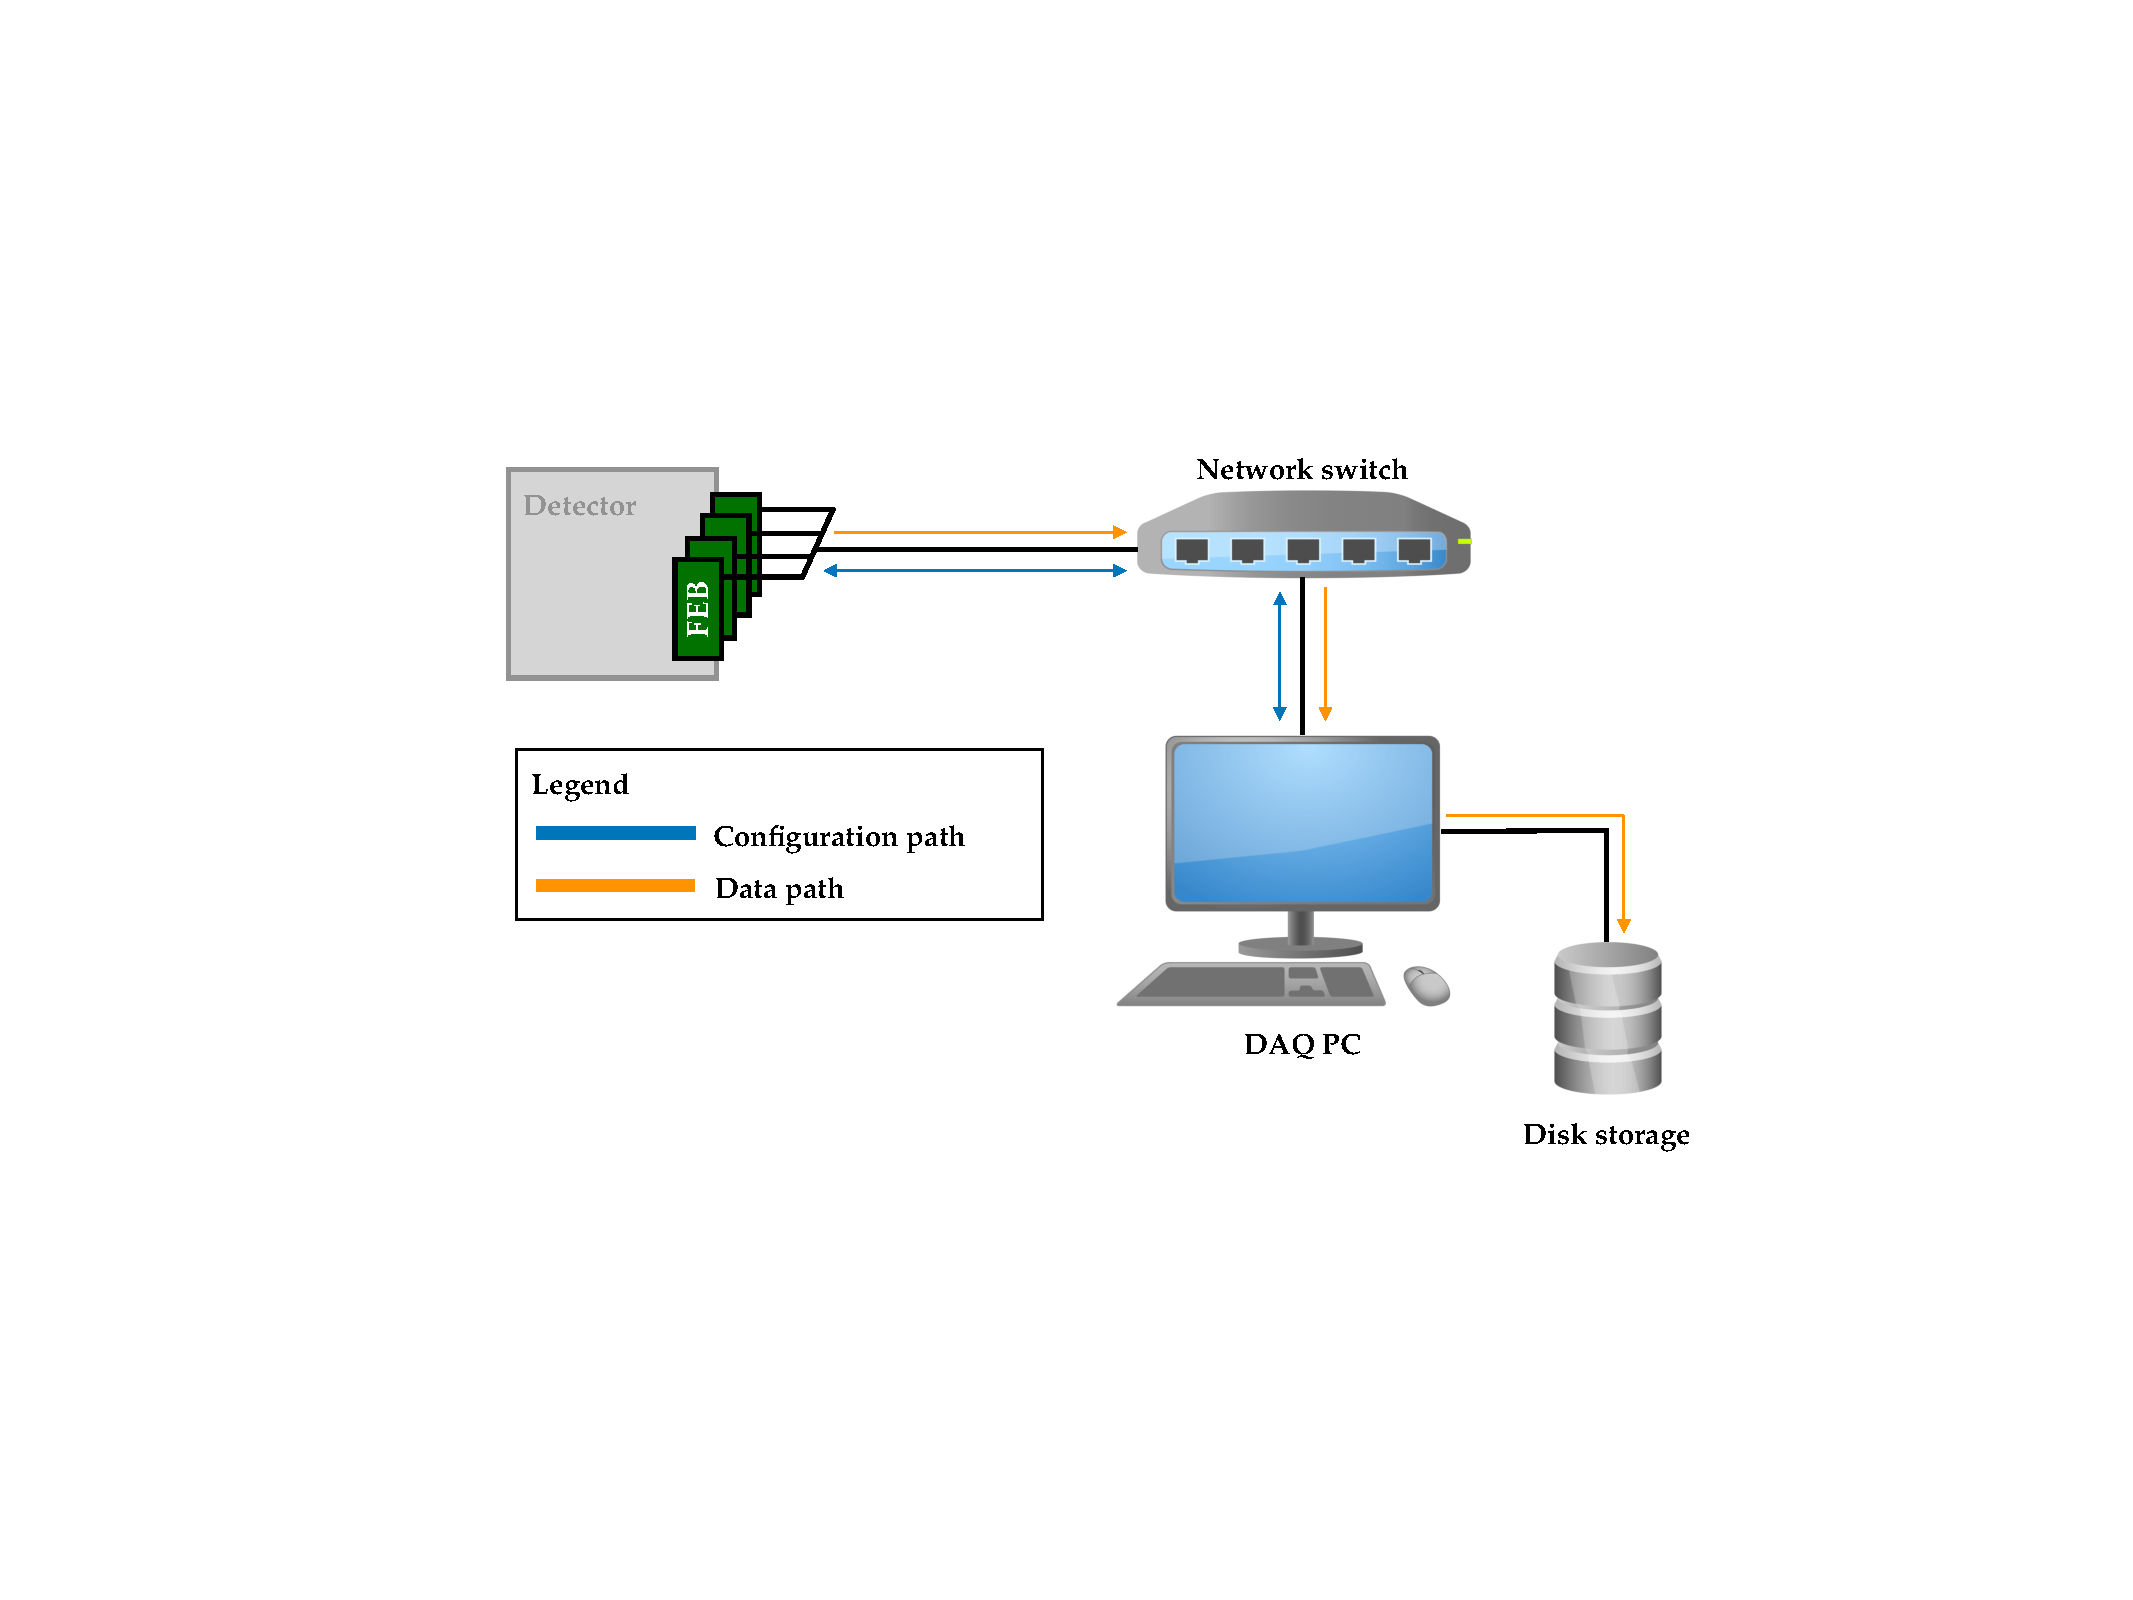
\includegraphics[width=0.5\textwidth]{figures/nsw/vrs/vrs_diagram_minimalPDF}
        \caption{
            A minimal VRS setup, in which a set of frontend boards (FEBs) are connected directly
            to the hosting DAQ PC.
            This setup is that typically used in labs and test benches, in which direct
            study of the VMM ASIC can be performed.
        }
        \label{fig:vrs_diagram_minimal}
    \end{center}
\end{figure}

\begin{figure}[!htb]
    \begin{center}
        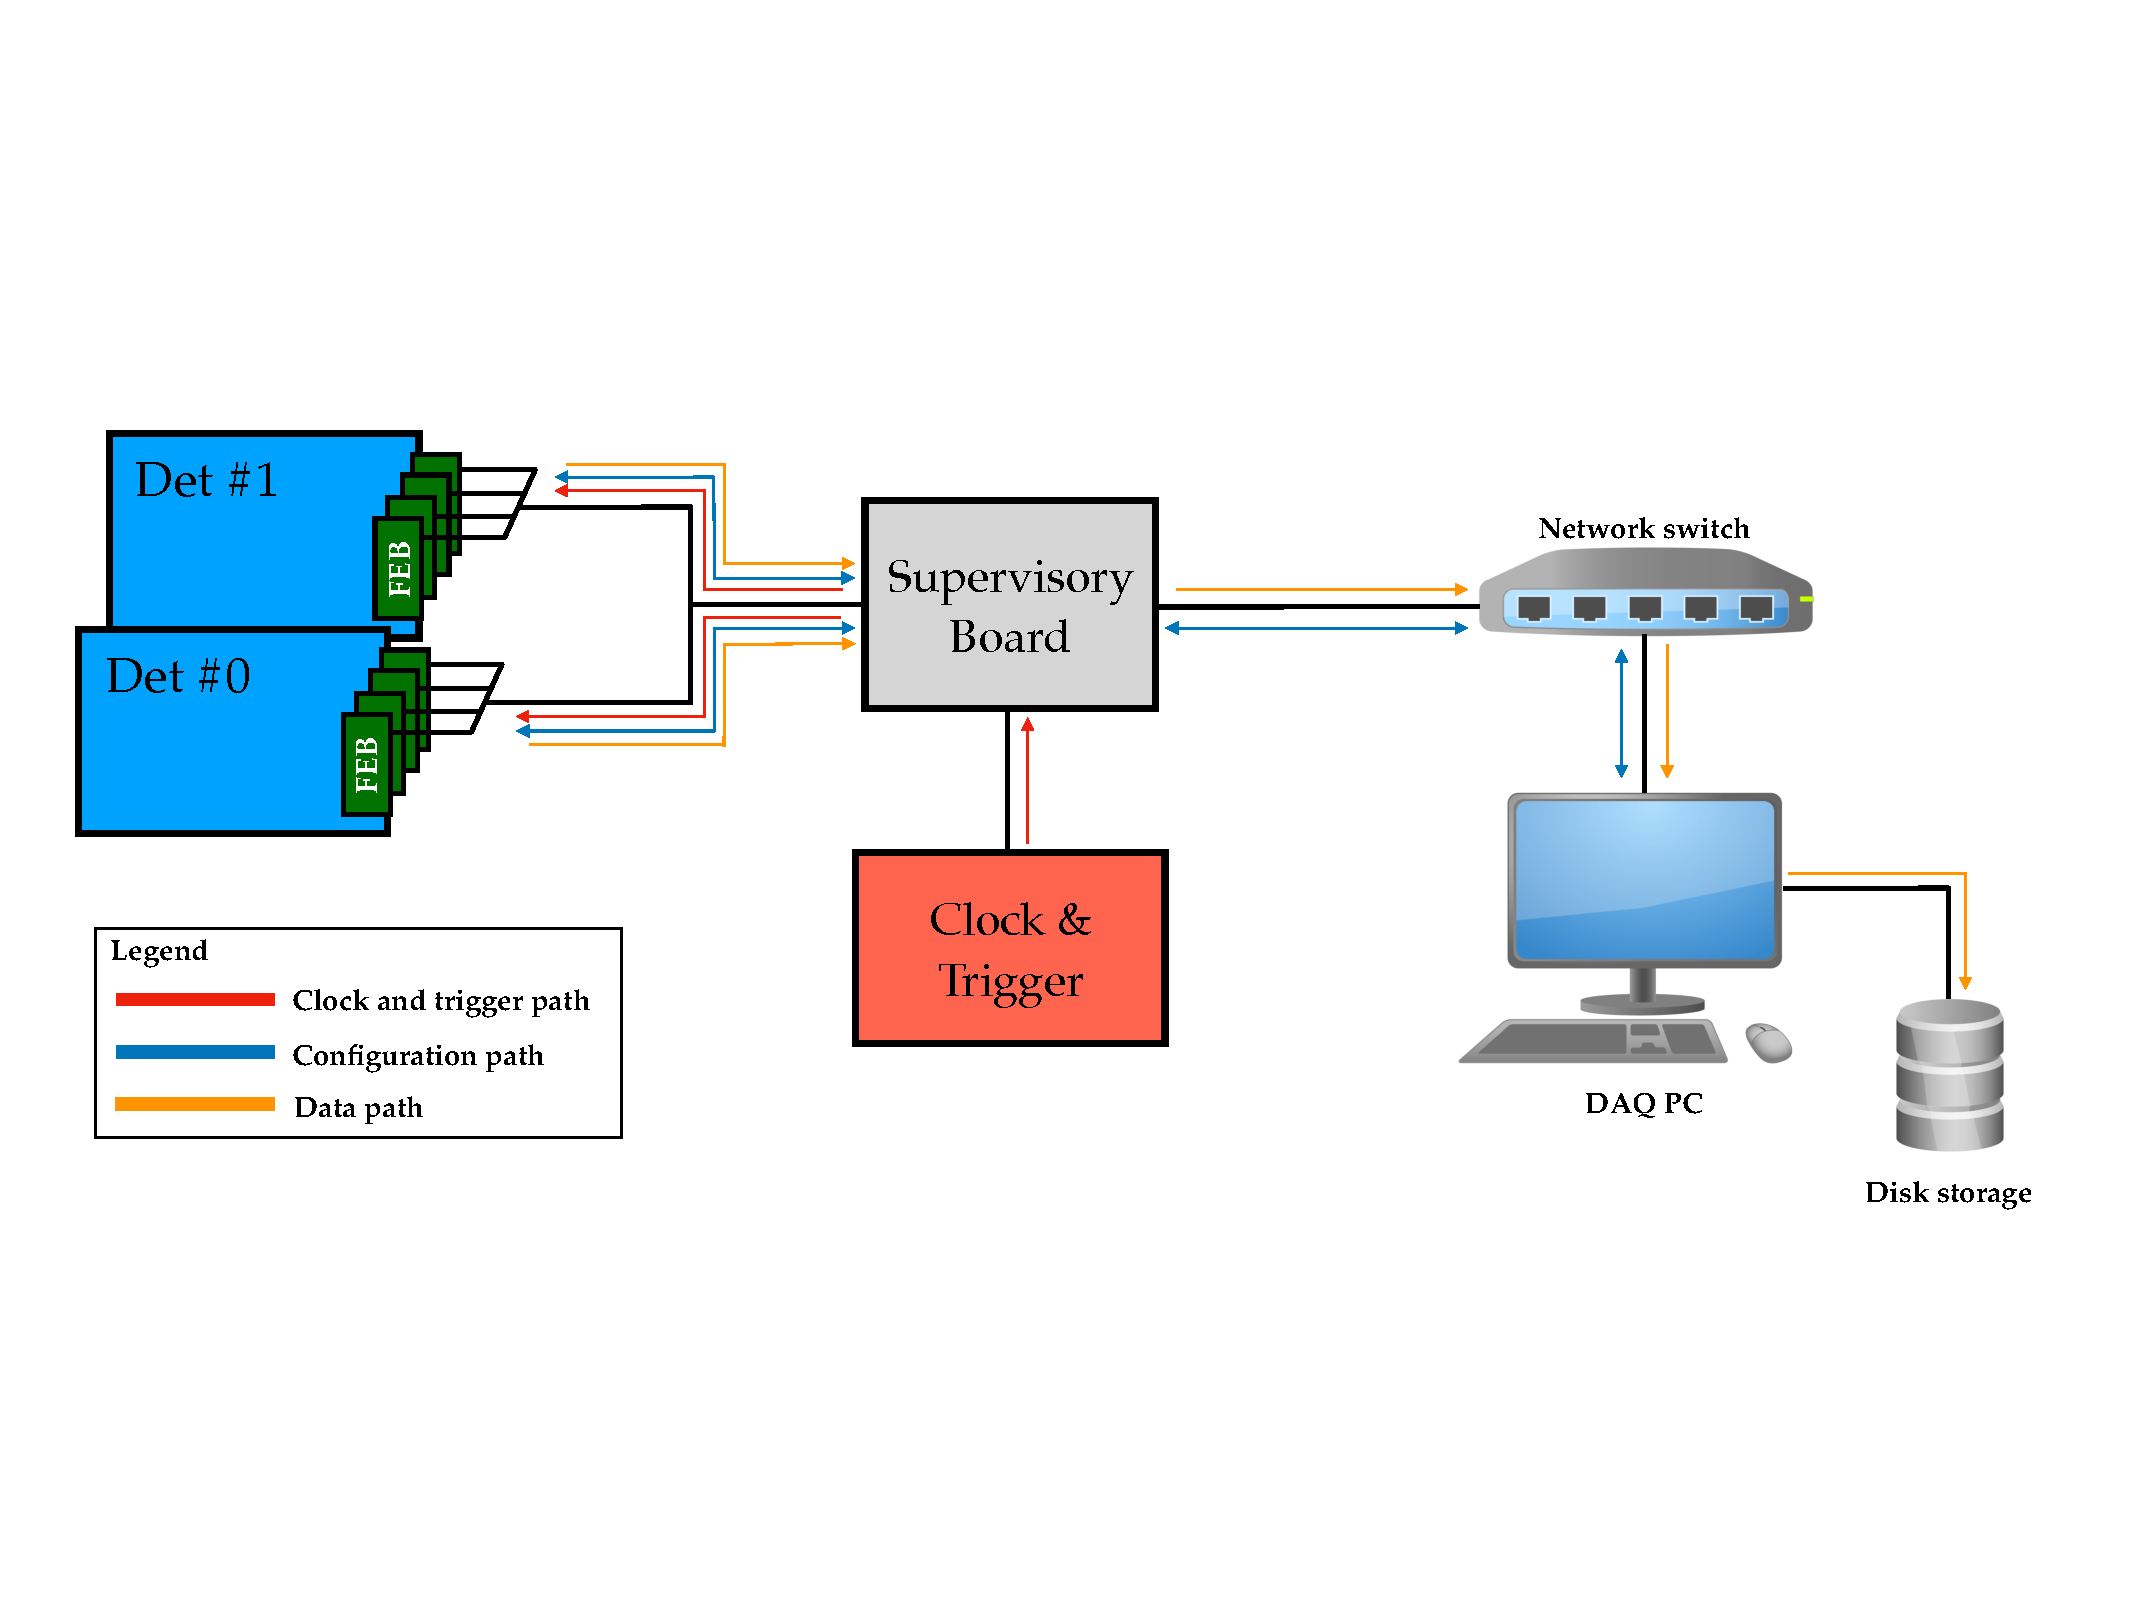
\includegraphics[width=0.7\textwidth]{figures/nsw/vrs/vrs_diagramPDF}
        \caption{
            A standard VRS setup, in which detector-grouped frontend boards (FEBs) receive external clock
            and trigger signals that are transmitted synchronously via the intermediate VRS Supervisory Board (VSB).
            This setup is used mainly for data taking scenarios in testbeams or in cosmic-ray stands.
        }
        \label{fig:vrs_diagram}
    \end{center}
\end{figure}
\FloatBarrier

%\subsection{VERSO}
%\label{sec:verso}

%\subsection{Calibration Algorithm Development}
%\label{sec:calib_alg}

%\subsubsection{Gain}
%\subsubsection{ADC Calibration}
%\subsubsection{Noise Measurements}
%\subsubsection{Timing Calibration}
%\subsubsection{Per-channel Threshold Equilisation}
